\section{Conception du Jeu Canvas}

Le jeu développé sur le Canvas HTML5 représente le rigeur de notre réflexion architecturale, se distinguant par une modularité exemplaire et une application forte des concepts de la programmation orientée objet. Afin de garantir des performances optimales et une grande facilité de maintenance, nous avons strictement séparé le moteur de jeu, la gestion de l'interface utilisateur, les calculs physiques et la logique métier. 

Le cœur du système est orchestré par une classe principale agissant comme un point d'entrée, qui délègue ensuite les responsabilités temporelles et spatiales à des gestionnaires spécialisés. Un gestionnaire de niveau s'occupe de l'instanciation des cartes et du placement des entités à partir de fichiers de configuration externes, tandis qu'un gestionnaire de tours régule le flux du combat et évalue en continu les conditions de victoire ou de défaite. En parallèle, un gestionnaire d'interface fait le pont entre les nécessités de rendu graphique sur le Canvas et les superpositions d'éléments HTML du DOM pour les menus et les barres d'outils.

% ==========================================
% INSERTION DU DIAGRAMME 1 : CORE ENGINE
% Ce diagramme illustre les relations entre Game, UIManager, LevelManager, etc.
% ==========================================
\FloatBarrier
\begin{figure}[H]
	\centering
	% Remplacez 'core_engine.png' par le nom exact de votre image exportée
	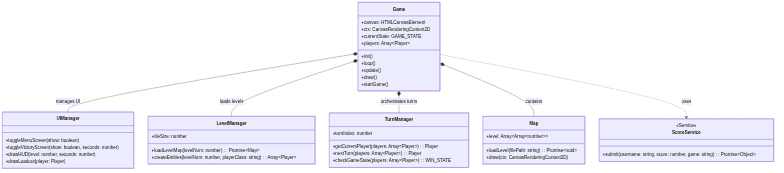
\includegraphics[width=1\textwidth]{canvas_1.png}
	\caption{Architecture du moteur principal et de ses gestionnaires}
	\label{fig:core_engine}
\end{figure}
\FloatBarrier

La hiérarchie des entités a été pensée pour maximiser la factorisation du code tout en permettant une grande diversité de comportements à l'écran. Toutes les entités physiques, qu'elles soient contrôlées par un joueur humain ou par l'ordinateur, héritent d'une classe de base abstraite définissant la physique spatiale, les règles de collisions environnementales et la gestion des points de vie. À partir de cette fondation solide, nous avons dérivé des classes spécifiques pour les joueurs humains, telles que l'archer ou le mage, ainsi que des classes distinctes pour les adversaires, comme les gobelins ou le dragon. Cette séparation claire des responsabilités structurelles permet d'ajouter de nouvelles classes de personnages de manière triviale, simplement en instanciant une nouvelle classe fille et en lui attribuant des statistiques ou des dimensions propres, sans risquer de perturber la physique fondamentale du jeu.

% ==========================================
% INSERTION DU DIAGRAMME 2 : HIÉRARCHIE DES ENTITÉS
% Ce diagramme montre l'héritage de GraphicalObject -> Player -> Bot / Archer / Mage, etc.
% ==========================================
\FloatBarrier
\begin{figure}[H]
	\centering
	% Remplacez 'entities.png' par le nom exact de votre image exportée
	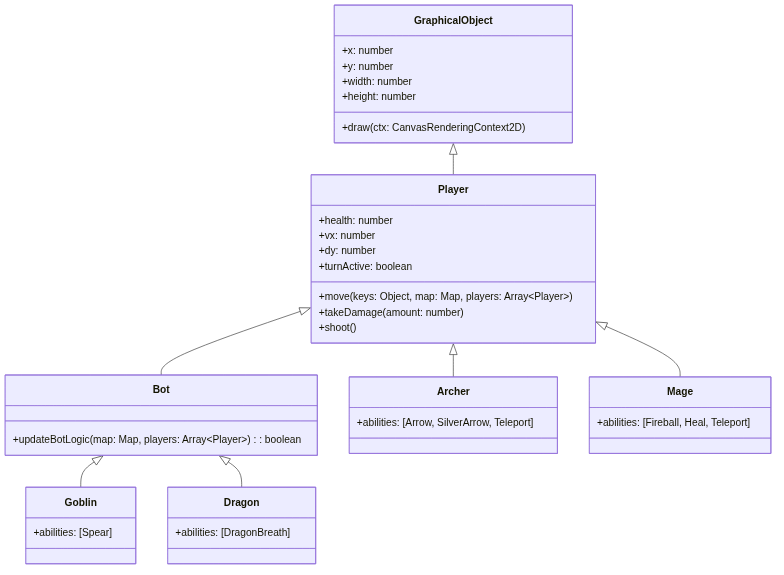
\includegraphics[width=1\textwidth]{canvas_2.png}
	\caption{Hiérarchie d'héritage des entités physiques (Joueurs et IA)}
	\label{fig:entities}
\end{figure}
\FloatBarrier

Le système d'armement et de projectiles suit une philosophie d'héritage similaire, garantissant une gestion unifiée de la balistique. Un objet projectile de base implémente les algorithmes de détection de collision et de cinématique linéaire dans un espace assujetti à la gravité. Des projectiles plus complexes viennent ensuite surcharger ces comportements de base. Par exemple, une boule de feu inclut une dissipation progressive des dégâts en fonction de la distance parcourue, tandis qu'une flèche en argent utilise l'identification de type à l'exécution pour infliger des dégâts critiques uniquement si la cible identifiée est un boss. Cette conception permet à la boucle principale du moteur de jeu de traiter et de dessiner tous les tirs de manière totalement agnostique, tout en laissant chaque projectile dicter ses propres règles de résolution lors de l'impact.

% ==========================================
% INSERTION DU DIAGRAMME 3 : SYSTÈME DE PROJECTILES
% Ce diagramme montre comment Projectile se décline en Arrow, Fireball, Spear, etc.
% ==========================================
\FloatBarrier
\begin{figure}[H]
	\centering
	% Remplacez 'projectiles.png' par le nom exact de votre image exportée
	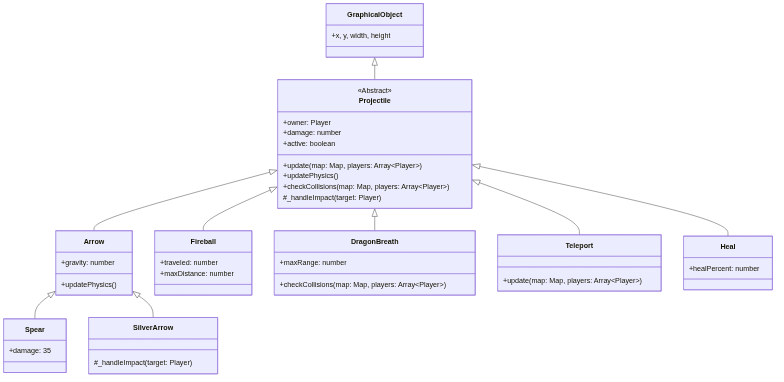
\includegraphics[width=1\textwidth]{canvas_3.png}
	\caption{Conception modulaire du système de balistique et des projectiles}
	\label{fig:projectiles}
\end{figure}
\FloatBarrier

Enfin, la véritable force de cette architecture réside dans l'utilisation de patrons de conception comportementaux éprouvés, notamment le patron Stratégie pour l'intelligence artificielle et le patron Commande pour le système de compétences. Plutôt que de coder en dur les prises de décision des ennemis dans leurs classes respectives, nous leur injectons dynamiquement une stratégie cognitive abstraite. Ainsi, un ennemi peut se voir assigner une intelligence basique se contentant de foncer en ligne droite, une intelligence avancée capable d'esquiver les obstacles et de prédire les chutes balistiques, ou encore une stratégie purement immobile. De manière analogue, toutes les actions des personnages sont encapsulées dans des classes de compétences indépendantes obéissant à une interface commune. Qu'il s'agisse de tirer une flèche physique, de lancer un sort de soin modifiant les statistiques internes, ou de se téléporter en manipulant les vecteurs spatiaux, chaque capacité gère de manière autonome son propre temps de recharge et son exécution. Ce paradigme rend l'ajout de nouvelles mécaniques de jeu extrêmement flexible, car les compétences sont totalement décorrélées de la logique interne des avatars qui les utilisent.

% ==========================================
% INSERTION DU DIAGRAMME 4 : PATRONS DE CONCEPTION
% Ce diagramme expose le pattern Strategy (AI) et Command (Abilities)
% ==========================================
\FloatBarrier
\begin{figure}[H]
	\centering
	% Remplacez 'patterns.png' par le nom exact de votre image exportée
	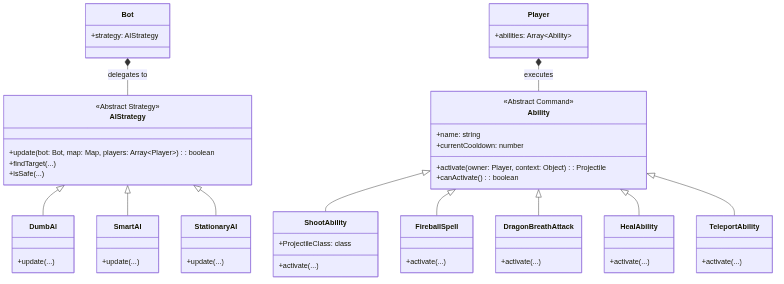
\includegraphics[width=1\textwidth]{canvas_4.png}
	\caption{Utilisation des patrons Stratégie (IA) et Commande (Compétences)}
	\label{fig:patterns}
\end{figure}
\FloatBarrier